\documentclass{article}
\usepackage{arxiv}
\usepackage[utf8]{inputenc} % allow utf-8 input
\usepackage[T1]{fontenc}    % use 8-bit T1 fonts
\usepackage{hyperref}       % hyperlinks
\usepackage{url}            % simple URL typesetting
\usepackage{booktabs}       % professional-quality tables
\usepackage{amsfonts}       % blackboard math symbols
\usepackage{nicefrac}       % compact symbols for 1/2, etc.
\usepackage{microtype}      % microtypography
\usepackage{lipsum}
\usepackage[]{algorithm2e}
\usepackage{graphicx}
\usepackage{enumitem}


\title{Hierarchical Leader Election Algorithm with Remoteness Constraint}


\author{
  P.~Kuznetsov \\
  INFRES Department\\
  Télécom ParisTech\\
  Paris, France \\
  \texttt{petr.kuznetsov@telecom-paristech.fr} \\
  \And
  A.~Diaconescu \\
  INFRES Department\\
  Télécom ParisTech\\
  Paris, France \\
  \texttt{ada.diaconescu@telecom-paristech.fr} \\
  \And
  M.~Tbarka \\
  Department of Software Engineering\\
  ENSIAS\\
  Rabat, Maroc \\
  \texttt{mohamed.tbarka@telecom-paristech.fr} \\
  %% \AND
  %% Coauthor \\
  %% Affiliation \\
  %% Address \\
  %% \texttt{email} \\
  %% \And
  %% Coauthor \\
  %% Affiliation \\
  %% Address \\
  %% \texttt{email} \\
  %% \And
  %% Coauthor \\
  %% Affiliation \\
  %% Address \\
  %% \texttt{email} \\
}

\begin{document}
\maketitle

\begin{abstract}
A hierarchical algorithm for electing a leaders' hierarchy in an asynchronous network with dynamically changing communication topology is presented including a remoteness's constraint towards each leader. The algorithm ensures that, no matter what pattern of topology changes occur, if topology changes cease, then eventually every connected component contains a unique leaders' hierarchy. The algorithm combines ideas from the Temporally Ordered Routing Algorithm (TORA) for mobile ad hoc networks with a wave algorithm, all within the framework of a height-based mechanism for reversing the logical direction of communication links. Moreover, an improvement from the algorithm in is the introduction of logical clocks as the nodes’ measure of time, instead of requiring them to have access to a common global time. This new feature makes the algorithm much more flexible and applicable to real situations, while still providing a correctness proof. It is also proved that in certain well behaved situations, a new leader is not elected unnecessarily.
\end{abstract}


% keywords can be removed
\keywords{leader election \and hierarchical algorithm}

\section{Introduction}
\paragraph{}Leader election is an important primitive for distributed computing, useful as a subroutine for any application that requires the selection of a unique processor among multiple candidate processors. Applications that need a leader range from the primary-backup approach to replication-based fault-tolerance to group communication systems \cite{1}, and from video conferencing to multi-player games \cite{8}.

\paragraph{}In a dynamic network, communication links go up and down frequently. Wireless mobile networks are one example of dynamic networks, since node mobility changes the communication topology continuously. Even if nodes do not move, wireless communications are subject to more interference than in the wired case, but wired networks can also experience frequent topology changes. Recent research has focused on porting some of the applications mentioned above to dynamic networks, including wireless and sensor networks. For instance, Wang and We propose a replication-based scheme for data delivery in mobile and fault-prone sensor networks \cite{24}. Thus there is a need for leader election algorithms that work in dynamic networks.

\paragraph{}We consider the problem of ensuring that, if link changes
cease, then eventually each connected component of the
network has a unique leader (introduced as the “local leader
election problem” in [5]). The algorithm in [10] is an exten-
sion of the leader election algorithm in [13], which in turn
is an extension of the MANET routing algorithm TORA in
[17]. TORA itself is based on ideas from [6]. Our cur-
rent algorithm relaxes the requirement in [10] of nodes hav-
ing perfect clocks and uses the concept of logical clocks
instead.

\paragraph{}Gafni and Bertsekas [6] present two routing algorithms
based on the notion of link reversal. In these algorithms,
each node maintains a height variable, drawn from a totally
ordered set; the link between two nodes is considered to be
directed from the endpoint with larger height to that with
smaller height. Whenever a node becomes a sink, i.e., has
no outgoing links, due to a link failure or due to notification
of a neighbor’s changed height, the node increases its height
so that at least one of its incoming links becomes outgoing.
In one of the algorithms of [6], the height is a pair, while in
the other the height is a triple; in both situations, heights are
compared lexicographically and the least significant com-
ponent is the node’s unique id.

\paragraph{}The algorithms in [6] cause an infinite number of mes-
sages to be sent if a portion of the graph is disconnected
from the destination. This drawback is overcome in TORA
[17], through the addition of a clever mechanism by which
nodes can identify that they have been partitioned from the
destination. In this case, the nodes go into a quiescent state.

\paragraph{}In TORA, each node maintains a 5-tuple of integers
for its height, consisting of, from left to right, a 3-tuple
called the reference level, a delta component, and the node’s
unique id. The height tuple of each node is lexicographi-
cally compared to the tuple of each neighbor to impose a
logical direction on links (higher tuple toward lower.

\paragraph{}The purpose of a non-zero reference level is to indicate
when nodes have lost their path to the destination. Initially,
the reference level is all zeroes. When a node loses its last
outgoing link due to a link disappearing, it starts a new ref-
erence level by changing the first component of the triple to
the current time, the second to its own id, and the third to 0,
meaning that the search for the destination is started. Refer-
ence levels are propagated throughout a connected compo-
nent, as nodes lose outgoing links, in a search for an alter-
nate directed path to the destination. Propagation of refer-
ence levels is done using a mechanism by which a node in-
creases its reference level when it becomes a sink; the delta
value of the height is manipulated to ensure that links are
oriented appropriately. If one section of the communication
graph is a dead-end, then the third component of the refer-
ence level triple is set to 1. When this happens, the reference
level is said to have been reflected, since it is subsequently
propagated back toward the originator. If the originator re-
ceives reflected reference levels back from all its neighbors,
then it has identified a partitioning from the destination.

\paragraph{}The key observation in [13] is that TORA can be adapted
for leader election: when a node detects that it has been
partitioned from the destination (the old leader), then, in-
stead of becoming quiescent, it elects itself. The informa-
tion about the new leader is then propagated through the
connected component. A sixth component was added to the
height tuple to record the leader’s id.

\paragraph{}However, when multiple topology changes occur, the al-
gorithm in [13] can fail. In [10], a modification to the al-
gorithm that works in an asynchronous system with arbi-
trary topology changes is presented. One new feature of
this algorithm is to add a seventh component to the height: a
timestamp associated with the leader id that records the time
that the leader was elected. Also, a new rule by which nodes
can choose new leaders is included. A newly elected leader
initiates a “wave” algorithm [22]: when different leader ids
collide at a node, the one with the most recent timestamp is
chosen as the winner and the newly adopted height is further
propagated. This strategy for breaking ties between com-
peting leaders makes the algorithm compact and elegant, as
messages sent between nodes carry only the height infor-
mation of the sending node, and every message is identical
in content.

\paragraph{}Another contribution of [10] is a relatively brief, yet
complete, proof of algorithm correctness. In addition to
showing that each connected component eventually has a
unique leader, it is shown that in certain well-behaved situ-
ations, a new leader is not elected unnecessarily. The proof
handles arbitrary asynchrony in the message delays.

\paragraph{}In this paper, we relax the requirement in [10] that nodes
have perfect clocks. Instead, we incorporate the idea of log-
ical clocks, introduced in [11] into the already existing al-
gorithm. In order to provide a way for logical clocks to be
updated, we introduce a timestamp to every message be-
ing sent. Thus, now besides the height as the data of the
message, we include an integer-valued timestamp. More-
over, we provide a correctness proof for the algorithm and
specific type of situations in which a leader is not elected
unnecessarily.

\newpage

\paragraph{}Leader election has been extensively studied, both for
static and dynamic networks, the latter category includ-
ing mobile networks. Here we mention some representa-
tive papers on leader election in dynamic networks. Hatzis
et al. [9] presented algorithms for leader election in mo-
bile networks in which nodes are expected to control their
movement in order to facilitate communication. This type
of algorithm is not suitable for networks in which nodes
can move arbitrarily. Vasudevan et al. [23] and Masum et
al. [15] developed leader election algorithms for mobile net-
works with the goal of electing as leader the node with the
highest priority according to some criterion. Both these al-
gorithms are designed for the broadcast model. In contrast,
our algorithm can elect any node as the leader, involves
fewer types of messages than either of these two algorithms,
and uses point-to-point communication rather than broad-
casting. Brunekreef et al. [2] devised a leader election
algorithm for a 1-hop wireless environment in which nodes
can crash and recover. Our algorithm is suited to an arbi-
trary communication topology.

\paragraph{}Several other leader election algorithms have been devel-
oped based on MANET routing algorithms. The algorithm
in [18] is based on the Zone Routing Protocol [7]. A cor-
rectness proof is given, but only for the synchronous case
assuming only one topology change. In [4], Derhab and
Badache present a leader election algorithm for ad hoc wire-
less networks that, like ours, is based on the algorithms pre-
sented by Malpani et al. [13]. Our algorithm is simpler and
uses fewer message types and smaller messages than the al-
gorithm presented by Derhab and Badache. Unlike Derhab
and Badache, we prove our algorithm is correct even when
communication is asynchronous and multiple link changes
and network partitions occur during the leader election pro-
cess.

\paragraph{}Dagdeviren et al. [3] and Rahman et al. [19] have re-
cently proposed leader election algorithms for mobile ad
hoc networks; these algorithms have been evaluated solely
through simulation, and lack correctness proofs. A differ-
ent direction is randomized leader election algorithms for
wireless networks (e.g., \cite{1}); our algorithm is deterministic.

\paragraph{}Fault-tolerant leader election algorithms have been proposed for wired networks. Representative examples are Mans and Santoro’s algorithm for loop graphs subject to permanent link failures \cite{14}, Singh’s algorithm for complete graphs subject to intermittent link failures \cite{20}, and Pan and Singh’s algorithm \cite{16} and Stoller’s algorithm \cite{21} that tolerate node crashes.

\section{Preliminaries}

\subsection{System Model}
We assume a system consisting of a set $P$ of computing nodes and a set $L$ of bidirectional communication links between nodes. $L$ consists of one link for each unordered pair of nodes, i.e., every possible link is represented. The nodes are assumed to be completely reliable. The links between nodes go up and down, due to the movement of the nodes. While a link is up, the communication across it is in first-in-first-out order and is reliable but asynchronous.

We model the whole system as a set of (infinite) state machines that interact through shared events (a specialization of the IOA model \cite{12}). Each node and each link is modeled as a separate state machine. The shared events are Link Up/Down notifications and receipt of messages, all of which are controlled and initiated by the link and responded to by the node. The sending of a message is also a shared event, but it is controlled and initiated by the node and responded to by the link; we are not explicitly modeling this.

The next subsection gives more details about how links are modeled and specifies the initial states. The algorithm executed by the nodes and its initial states are described in Section 3.
\subsection{Modeling Asynchronous Dynamic Links}
We now specify how communication is assumed to occur over the dynamic links, and how notification of a link’s status is synchronized at the two endpoints of the link.

The state of a link $Link_{u, v}$, which models the bidirectional communication link between node u and node v, consists of a status variable and two queues of messages.

The possible values of the status variable are $Up$, $GoingDown_{u}$ , $GoingDown_{v}$, $Down$, $ComingUp_{u}$, and $ComingUp_{v}$. The link transitions among different values of its status variable through $LinkUp$ and $LinkDown$ events. Figure 1 shows the state transition diagram for $Link_{u, v}$. The intuition is that if a $LinkUp$ (resp., $LinkDown$) occurs at one endpoint of the link, then $LinkUp$ (resp., $LinkDown$) must occur at the other endpoint before $LinkDown$ (resp., $LinkUp$) can occur at either end.

The other components of the link’s local state are the two message queues: $mqueue_{u,v}$ holds messages in transit from $u$ to $v$ and $mqueue_{v,u}$ holds messages in transit from $v$ to $u$.

An attempt by node $u$ to send a message to node $v$ results in the message being appended to $mqueue_{u,v}$ if the link’s status is either $ComingUp_u$ or $Up$; otherwise there is no effect.

\begin{figure}[hbtp]
\centering
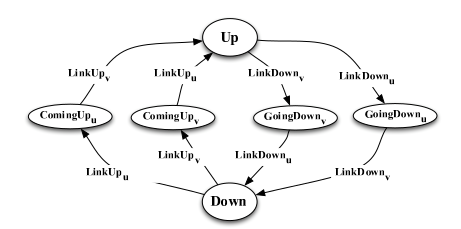
\includegraphics[scale=.6]{screenshot.png}
\caption{State diagram for status variable of $Link_{u, v}$.}
\end{figure}

If the status is $ComingUp_u$ , then messages in transit from $u$ to $v$ are held in the queue until $v$ has been notified that the link is $Up$. Once the link is $Up$, the event by which node $u$ receives the message at the head of $mqueue_{v,u}$ is enabled to occur. An attempt by node $v$ to send a message to node $u$ is handled analogously.

Whenever a $LinkDown_u$ or $LinkDown_v$ event occurs, both message queues are emptied. Neither $u$ nor $v$ is alerted to which messages in transit have been lost due to the $LinkDown$.

In an initial state of the link, both message queues are empty and the status is either $Up$ or $Down$.

\subsection{Configurations and Executions}
The notion of configuration is used to capture an instantaneous snapshot of the state of the entire system. A configuration is a vector of node states, one for each node in $P$, and a vector of link states, one for each link in $L$.
Assume that the undirected graph $G = (V, E)$ defines the initial communication topology of the system, where $V$ is a set of vertices corresponding to the set $P$ of nodes, and E is a set of edges corresponding to the set of communication links that are up. In an initial configuration with respect to $G$, each node is in an initial state (as prescribed by the node’s algorithm), each link corresponding to an edge in $E$ is in an initial state with its status equal to Up, and every other link has its status equal to Down.
Define an execution as an infinite sequence $C_0, e_1 ,C_1, e_2 ,C_2, ...$ of alternating configurations and events, starting with an initial configuration and, if finite, ending with a configuration, that satisfies the following safety conditions:
\begin{itemize}
\item $C_0$ is an initial configuration (w.r.t. some initial topology $G$).
\item The preconditions for event are true in $C_{i-1}$ for all $i\geq 1$.
\item $C_i$ is the result of executing event $e_i$ on configuration $C_{i - 1}$ , for all $i \geq 1$ (only the node and link involved in an event change state, and they change according to their state machine transitions).
\end{itemize}

An execution also satisfies the following liveness conditions:
\begin{itemize}
\item If a link remains Up for infinitely long, then every message sent over the link is eventually delivered.
\item For each link, if only a finite number of link events occur, then the link status after the last one is either Up or Down (not in between).
\end{itemize}

We also assign a positive real-valued global time gt to each event $e_i$, $i ≥ 1$, such that $gt(e_i) < gt(e_{i + 1}^)$ and, if the execution is infinite, the global times increase without bound. Each configuration inherits the global time of its preceding event, so $gt(C_i) = gt(e_i)$ for $i \geq 1$; we define $gt(C_0)$ to be $0$. We assume that the nodes do not have access to $gt$.

\subsection{Problem Definition}
Each node u in the system has a local variable $lid_{u}$ to hold the identifier of the node currently considered by u to be the supreme leaders of the connected component containing u, and another local variable $slid_u$ to hold the identifier of the node currently considered by u to be the sub-leader in such a way that the distance to this subèleader does not exceed a certain constant d (the remoteness constraint). The set of all the leaders including the supreme one forms a spanning tree as subgraph of the DAG established.
In every execution that includes a finite number of topology changes, we require that the following eventually holds:
\begin{itemize}
\item Every connected component $CC$ of the final topology contains a node $l$, the supreme leader, such that $l$ is the only node which verifies $ lid_{l} = l $.
\item For each node u of each component $CC$, different from the supreme leader, a node v exists such as $slid_{u} = v$ and $d_{u,v} < D$ ($D$ is the maximum remoteness towards a leader and the $ d_{u,v} $ is the shortest distance between $u$ and $v$)
\end{itemize}

In a more formal way, one can state the problem as follows:\\
In every execution that includes a finite number of topology changes, we require that the following eventually holds:

\begin{itemize}
\item For each node $u$ of every connected component $CC$ of the final topology:
$u$ selects $(slid_u, pre_u)$, ${(slid_u, pre_u) \in N_u \times N_u}$ such that ${(slid_u, pred_u)}_{u \in CC}$ is a spanning tree $T$ ($slid_u$ (resp. $pred_u$) is the sub-leader (resp. the predecessor to reach $lid_u$) considered as such by i.
\item For each node $u$, different from the root of $T$, of every connected component $CC$ of the final topology:\\
if $ (k-1)D < depth_T (i) <= kD, k \in IN $, then $ depth_T(lid_i)=(k-1)D$ ($depth_T(u)$ is the depth of u in T)
\end{itemize}



Our algorithm also ensures that eventually each link in the system has a direction imposed on it by virtue of the data stored at each endpoint such that each connected component CC is a leader-oriented DAG containing a spanning tree, i.e., every node has a directed path to its local leader respecting, among the other leaders, a certain hierarchy containing one supreme leader.

\newpage

\section{Hierarchical Leader Election Algorithm}
\newpage
\subsection{Informal Description}
\paragraph{}Each node in the system has a 7-tuple of integers called a height and another 2-tuple of integers called sub-leader pair. The directions of the edges in the graph are determined by comparing the heights of neighboring nodes: an edge is directed from a node with a larger height to a node with a smaller height. The spanning tree is defined using the sub-leader pairs: each sub-leader's id defines a certain level of hierarchy of the concerned spanning tree and each predecessor defines how move on through the spanning tree. Due to topology changes nodes may lose some of their incident links, or get new ones throughout the execution. Whenever a node loses its last outgoing link because of a topology change, it has no path to the current leader, so it reverses all of its incident edges. Reversing all incident edges acts as the start of a search mechanism (called a reference level) for the current leader. Each node that receives the newly started reference level reverses the edges to some of its neighbors and in effect propagates the search throughout the connected component. Once a node becomes a sink and all of its neighbors are already participating in the same search, it means that the search has hit a dead end and the current leader is not present in this part of the connected component. Such dead-end information is then propagated back towards the originator of the search. When a node which started a search receives such dead-end messages from all of its neighbors, it concludes that the current leader is not present in the connected component, and so the originator of the search elects itself as the new leader. Finally, this new leader information propagates throughout the network via an extra “wave” of propagation of messages.
\paragraph{}In our algorithm, two of the components of a node’s height are timestamps recording the time when a new “search” for the leader is started, and the time when a leader is elected. In the algorithm in [15], these timestamps are obtained from a global clock accessible to all nodes in the system. In this paper, we use the notion of causal clocks (defined in Section 2.3) instead.
\paragraph{}One difficulty that arises in solving leader election in dynamic networks is dealing with the partitioning and merging of connected components. For example, when a connected component is partitioned from the current leader due to links going down, the above algorithm ensures that a new leader is elected using the mechanism of waves searching for the leader and converge-casting back to the originator. On the other hand, it is also possible that two connected components merge together resulting in two leaders in the new connected component. When the different heights of the two leaders are being propagated in the new connected component, eventually, some node needs to compare both and decide which one to adopt and continue propagating. Recall that when a new leader is elected, a component of the height of the leader records the time of the election which can be used =to determine the more recent of two elections. Therefore, when a node receives a height with a different leader information from its own, it adopts the one corresponding to the more recent election.
\paragraph{}Similarly, if two reference levels are being propagated in the same connected component, whenever a node receives a height with a reference level different from its current one, it adopts the reference level with the more recent timestamp and continues propagating it. Therefore, even though conflicting information may be propagating in the same connected component, eventually the algorithm ensures that as long as topology changes stop, each connected component has a unique leader.
\newpage
In this section, we explain the local variables used in our leader election algorithm. The pseudocode for the algorithm is presented in Figures 2, 3 and 4. An overview and sample execution is given in Section 3.1. In the analysis, variable $v$ of node $i$ will be indicated as $v_i$.

Each node $i$ keeps an array of heights, $height_i$, with an entry for itself and for each of its neighbors, in which it stores the most recent height information that it has received for those nodes. Each height is a 7-tuple, with the following components:
\begin{enumerate}
\item $\tau$ , a nonnegative timestamp that is either 0 or the time when the current search for an alternate path to the leader was initiated
\item $oid$, a nonnegative value that is either 0 or the id of the node that started the current search
\item $r$, a bit that is set to 0 when the current search is initiated and set to 1 when the current search hits a deadend
\item $\delta$ , an integer that is set to ensure that links are directed appropriately to neighbors with the same first three components
\item $nlts$, a nonpositive timestamp whose absolute value is the time when the current leader was elected
\item $lid$, the id of the current leader
\item $id$, the id of the node
\end{enumerate}

In addition to $height_i$, $i$ keeps another height which is a 2-tuple, with the following components:
\begin{enumerate}
\item $slid$, the id of the sub-leader
\item $pred$, the id of the predecessor in the spanning tree
\end{enumerate}


Components $(\tau, oid, r)$ are referred to as the reference level, or $RL$; $(\tau , oid)$ alone are referred to as the reference level prefix; and $(nlts, lid)$ is referred to as the leader pair or $LP$. The components of entry $k$ in $height_i$ are referred to as $(\tau _k , oid_k, r_k, \delta _k, nlts_k, lid_k, k)$ in the pseudocode.

The height $(slid, pred)$ is referred to as the sub-leader pair, or $SLP$. The sub-leader pair of a node $i$ is referred to as $SLP_i$.

Nodes communicate over links during the algorithm execution by sending Update messages. Each message contains the height tuple and the logical clock timestamp of the sending node. The link between node $i$ and one of its neighboring nodes $j$ is considered by $i$ to be outgoing (directed from $i$ to $j$) if and only if $height_i[i] > height_i[j]$. That is, node $i$ uses the information in its local state concerning itself and node $j$ to determine (its view of) the direction of the link to $j$. Because of message delays, it is not necessarily the case that $i$ and $j$ have consistent views of the direction of the link between them.

Other events that occur at a node are formations \textit{(LinkUps)} and failures \textit{(LinkDowns)} of links. Suppose the most recent indication that node $i$ has received concerning the link between itself and node $j$ is a \textit{LinkUp}. If $i$ has received a message from $j$ since that \textit{LinkUp}, then $i$ considers $j$ as one of its neighbors, and stores the $id$ of $j$ in its local variable $N_i$. If $i$ has not yet received a message from $j$, then the link is considered as still forming, and $i$ stores the $id$ of $j$ in its local variable $forming_i$; $j$ is not considered a neighbor of $i$ (yet).

Nodes have no access to global time, but, instead, each of them has a local logical clock \cite{11}. A logical clock is a non-negative integer, initially 0. Logical clocks can be updated in two possible ways, depending on the type of the event occurring at a node. If a \textit{LinkUp} or a \textit{LinkDown} event occurs at a node, its logical clock is incremented by 1. Otherwise, if a node receives an Update message, the logical clock is set to one more than the maximum of the node’s current logical clock value and the timestamp included in the message. This way, we ensure that for each node, the value of its logical clock is non-decreasing for each subsequent event. The logical clock of a node is referred to as $LC$ in the pseudocode.
\newpage
Given an initial connected communication graph $G = (V, E)$, with $V$ corresponding to the set of nodes and $E$ to the set of communication links that are up, the initial state of each node $i$ is defined as follows \footnote{If initial knowledge of neighboring nodes is not available, then the algorithm could begin with each node in a singleton connected component.}.
\begin{itemize}
\item $forming_i$ is empty
\item $N_i$ contains the $id$ of every node $j$ such that the vertices in $V$ corresponding to $i$ and $j$ are neighbors in G
\item $height_i[i] = (0, 0, 0, \delta _i, 0, l, i)$, where $l$ is the $id$ of a fixed node in $i$’s connected component, the current leader
\item for each neighbor $j$ of $i$, $height_i[j] = height_j[j]$ (i.e., $i$ has accurate information about $j’s$ height)
\item $LC_i = 0$ (i.e. the logical clocks of all nodes are initially set to 0).
\end{itemize}

Furthermore, for each node $i$, $\delta _i$ equals the distance from $i$ to $l$; this condition ensures that every node has a directed path to $l$.

Next we define the conditions under which a node considers itself to be a sink.
\begin{itemize}
\item $SINK = ((LP_i ^j = LP_i ^i, \quad \forall j \in N_i)$ and $(height_i[i] < min \lbrace height_i[j],\quad \forall j \in N_i \rbrace)$ and $(lid_i ^i \neq i)).$
This predicate is true when, according to $i’s$ local state, $i$ is not a leader, has all neighbors with the same $LP$, and has no outgoing links. If node $i$ has links to any neighbors with different $LPs$, $i$ is not considered a sink, regardless of the directions of those links.
\end{itemize}


\subsection{Overview of Algorithm}
We depict the network as a DAG in which each bidirectional communication link points from a node with lexicographically higher height to another node with lexicographically lower height. Nodes send algorithm messages only when they change the contents of their height tuple. The contents of the height tuple at a particular node are changed only when the node elects itself a leader, when it changes its current leader, or when it loses its last outgoing link to its current leader. The network is quiescent when there is no message in transit on any link. Messages that do not cause a node to lose its last outgoing link to its current leader or to change its current leader result only in a change to the internal data that node keeps about its neighbors’ heights. Figure 5 shows a sample execution of the algorithm. Each part (a)–(l) is discussed below.
\begin{enumerate}[label=\alph *)]

\item A quiescent network is a leader-oriented DAG in which node H is the current leader. The height of each node is displayed in parenthesis. Link direction in this figure is shown using solid-headed arrows and messages in transit are arrows with outlined heads super-imposed on the links that point from message sender to receiver. The spanning tree is shown using green dotted link and the sub-leaders are represented by green circles.

\item When non-leader node G loses its last outgoing link due to the loss of the link to node H, G increments
its logical clock by 1, executes subroutine $STARTNEWREFLEVEL$ and takes on $RL(1,G,0)$, $\delta = 0$ and $SLP(-1,-1)$.
Then node $G$ sends messages with its new height to all its neighbors. By raising its height in this way, G has started a search for leader H.

\item Nodes D, E, and F receive the messages sent from node G, messages that cause each of these nodes to take on
$RL(1,G,0)$ and $SLP(-1,-1)$, set its $\delta $ to $−1$, ensuring that its height is lower than G’s but higher than the other neighbors’. Moreover, each of these nodes also updates its logical clock to 2. Then D, E and F send messages to their neighbors.

\item Node B has received messages from both E and D with the new $RL(1,G,0)$, and C has received a message
from F with $RL(1,G,0)$; as a result, B and C take on $RL(1,G,0)$ and $SLP(-1,-1)$ with $\delta $set to $−2$, update their logical clocks to 3 and send messages. Additionally, as a result of the messages sent by D, E, and F, node G updates its logical clock to 3.

\item Node A has received message from both nodes B and C. In this situation, node A is connected only to nodes that are participating in the search started by node G for leader H. In this case, node A “reflects” the search by setting the reflection bit in the $(1,G,*)$ reference level to 1, taking on $SLP(-1,-1)$, resetting its $\delta $ to 0, and sending its new height to its neighbors. Moreover, nodes A, D, E, and F update their clocks to 4.

\item Nodes B and C take on the reflected reference level $(1,G,1)$ and set their $\delta $ to −1, causing their heights to be lower than A’s and higher than their other neighbors’. They also update their logical clocks to 5 and send their new heights to their neighbors.

\newpage

\item Nodes D, E, and F act similarly as B and C did in part (f), but set their $\delta $ variables to −2. As a result from the messages sent by B and C, nodes A, D, E, and F update their logical clocks to 6.

\item  ,i), j), k), l) When node G receives the reflected reference level from all its neighbors, it knows that its search for H is in vain. G updates its logical clock to 7 and then elects itself. The new $SLP(G,-1)$ is adopted and the new $LP(-7,G)$ then propagates through the component, updating nodes’ logical clocks and sub-leader pairs along the way , assuming no further link changes occur; eventually each node has RL(0,0,0) and LP (-7,G), with D, E and F having $\delta = 1$ and $SLP(G,G)$, B and C having $\delta = 2$ and, respectively, $SLP(G,D)$ and $SLP(G,F)$, and A having $\delta = 3$ and $SLP(B,B)$.

\end{enumerate}
\newpage
\begin{figure}

\textbf{When node $u$ receives $Update(h)$ from node $v \in forming \cup N:$}
\\ \quad \quad // if v is in neither forming nor N, message is ignored
\begin{enumerate}
\item \quad $LC := LC + 1$   \textit{// increment logical clock}
\item \quad$height[v] := h$
\item \quad$forming := forming \setminus \lbrace v\rbrace$
\item \quad$N := N \cup \lbrace v\rbrace$
\item \quad$myOldHeight := height[u]$
\item \quad \textbf{if}($(nlts^u ,lid^u ) = (nlts^v ,lid^v ))$) // leader pairs are the same
\item \quad \quad \textbf{if}(SINK)
\item \quad \quad \quad \textbf{if}($\exists (\tau , oid, r)\quad | \quad (\tau ^k, oid^k, r^k) = (\tau , oid, r) ,\quad \forall k \in N $)
\item \quad \quad \quad \quad \textbf{if}($(\tau > 0)$ \textbf{and} $(r = 0)$)
\item \quad \quad \quad \quad \quad $REFLETREFLEVEL$
\item \quad \quad \quad \quad \textbf{else if} ($(\tau > 0)\quad \textbf{and} \quad (r = 1)\quad \textbf{and} \quad (oid = i)$)
\item \quad \quad \quad \quad \quad $ELECTSELF$
\item \quad \quad \quad \quad  \textbf{else}
\\ // ($\tau = 0$) or ($\tau >0$ and $r=1$ and $oid \neq i$)
\item \quad \quad \quad \quad \quad $STARTNEWREFLEVEL$
\item \quad \quad \quad \quad  \textbf{end if}
\item \quad \quad \quad \textbf{end if}
\item \quad \quad \textbf{else}
\\ // neighbors have different ref levels
\item \quad \quad \quad $PROPAGATELARGESTREFLEVEL$
\item \quad \quad \textbf{end if}
\\ \qquad // else not sink, do nothing
\item \quad \textbf{end if}
\item else // leader pairs are different
\item \quad $ADOPTLPIFPRIORITY(j,D)$
\item  \textbf{end if}
\item \textbf{if}($myOldHeight \neq height[i]$)
\item \quad send Update($height[i]$)
\item \quad with timestamp $LC$ to all $k \in (N \cup forming)$
\item \textbf{end if}
\end{enumerate}
\caption{Code triggered by Update message.}
\end{figure}

\newpage
\begin{figure}[hbtp]
\textbf{When $ChannelDown_{uv}$ event occurs}

\begin{enumerate}
\item \quad $LC := LC + 1$   \textit{// increment logical clock}
\item \quad $ N := N\backslash \left\lbrace v\right\rbrace $
\item \quad $ forming := forming \backslash \left\lbrace v\right\rbrace $
\item \quad \textbf{if} $ (N = \emptyset )$
\item \quad \quad $ELECTSELF$
\item \quad \quad send Update($heigth[u]$) to all $ w\in forming$
\item \quad \textbf{else if}(SINK)
\item \quad \quad $STARTNEWREFLEVEL$
\item \quad \quad send Update($heigth[u]$) to all $w\in (N \cup forming)$
\item \quad \textbf{else if} $(j=pred_i)$
\item \quad \quad $pred_i=min \left\lbrace k \quad \vert \quad k\in N_i \quad and \quad \delta_k = \delta_j \right\rbrace$
\item \quad \textbf{end if}
\end{enumerate}


\textbf{When $ChannelUp_{uv}$ event occurs}

\begin{enumerate}
\item \quad $LC := LC + 1$   \textit{// increment logical clock}
\item \quad $forming := forming \cup {v}$
\item \quad send Update($height[u]$) to all $ w \in (N \cup forming)$
\end{enumerate}
\caption{Code triggered by link change}
\end{figure}

\begin{figure}[hbtp]

\textbf{ELECTSELF}
\begin{enumerate}
\item $ height[i] := (0,0,0,0,-LC_{i},i,i) $
\item $SLP_i := (i,-1)$
\end{enumerate}

\textbf{REFLECTREFLEVEL}
\begin{enumerate}
\item $ height[i] := (\tau ,oid,1,0,nlts^{i},lid^i,i)$
\item $SLP_i := (-1,-1)$
\end{enumerate}


\textbf{PROPAGATELARGESTREFLEVEL}
\begin{enumerate}
\item $ (\tau , oid^{i}, r^{i}) := max\left\lbrace (\tau ^{k},oid^{k},r^{k}) \vert k\in N\right\rbrace  $
\item $ \delta ^{i} := min \left\lbrace \delta ^{k} \quad \vert \quad k \in N \quad and \quad (\tau ^{i} , oid^{i}, r^{i}) = (\tau ^{k},oid^{k},r^{k})\right\rbrace - 1 $
\item $SLP_i := (-1,-1)$
\end{enumerate}

\textbf {STARTNEWREFLEVEL}
\begin{enumerate}
\item $ height[i] := (\tau ,oid,1,0,nlts^{i},lid^i,i) $
\end{enumerate}

\textbf {ADOPTLPIFPRIORITY($j, D$)}
\begin{enumerate}
\item \textbf{if}$( (nlts^{j}<nlts^{i})\quad \textbf{or} \quad ((nlts^{j}=nlts^{i}) \quad \textbf{and} \quad (lid^{j} < lid^{i}))$
\item  \quad $ height[i] := (\tau ^{j} ,oid^{j},r^{j},\delta ^{j}+1,nlts^{j},lid^j,i) $

\item \quad \textbf{if} $ (\delta _{v} \quad mod \quad D \neq 0) $
\item \quad \quad $ SLP_u = (lid^j, min \left\lbrace k \quad \vert \quad k\in N_i \quad and \quad \delta_k = \delta_j \right\rbrace  )$
\item \quad \textbf{else if } $ \delta_v = 0 $
\item \quad \quad $ SLP_u = (j, -1)$
\item \quad \textbf{else}
\item \quad \quad $ SLP_u = (j, j)$
\item \quad \textbf{end if}
\item \textbf{end if}
\end{enumerate}

\caption{Subroutines}

\end{figure}

\clearpage

\begin{figure}[hbtp]
\centering
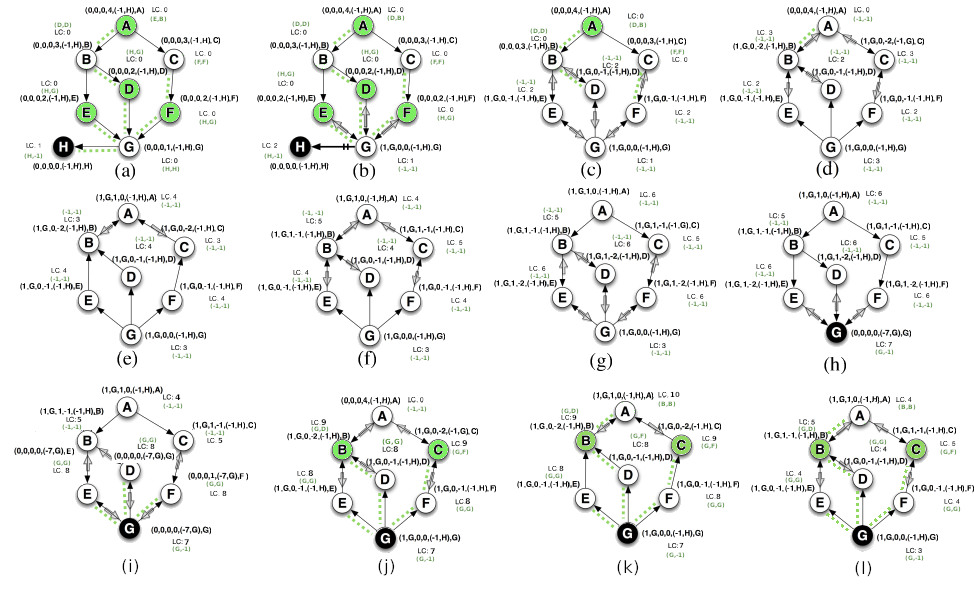
\includegraphics[scale=.5]{sample_execution.png}
\caption{Simple execution when leader H becomes disconnected (a), with time increasing from (a)–
(l). With no other link changes, every node in the connected component will eventually adopt G as its leader and a new leaders' hierarchy will be established.}
\end{figure}

\clearpage

\section{Correctness}

\paragraph{}
 
In this section\footnote{The correctness is intact regarding the Jennifer s paper}, we show that, once topology changes cease, the algorithm eventually terminates with each connected component forming a leader-oriented DAG. First, we make some definitions regarding the information concerning nodes’ heights that exists in the system and prove some properties about it. Then we prove that, after the last topology change, each node elects itself a finite number of times and a finite number of new reference levels are started. As a result, we show that eventually no messages are in transit and at that point we have a leader-oriented DAG.
\paragraph{}
Throughout the proof, consider an arbitrary execution of the algorithm in which the last topology change occurs at some time $t_{LTC}$ , and consider any connected component of the final topology.

\subsection{Height Tokens and Their Properties}
Since a node makes algorithm decisions based solely on comparisons of its neighboring nodes’ height tuples, we first present several important properties of the tuple contents.

Let $LC_u(t)$ be the logical clock value of node $u$ at time $t$. Define $h$ to be a height token for node $u$ in configuration if $h$ is in an Update message in transit from $u$, or $h$ is the entry for $u$ in the height array of $u$ or one of $u$’s neighbors.

Let $LP(h)$ be the leader pair of $h$, $RL(h)$ the reference level (triple) of $h$, $\delta (h)$ the $\delta$ value of $h$, $lts(h)$ the absolute value of the (nonpositive) leader timestamp (component $nlts$) of $h$, and $\tau (h)$ the $\tau $ value of $h$. For each configuration $C_i$ of the execution, recall from Sect. 2 that $gt(C_i)$ is the global time of its preceding event, $e_i$.

Given a configuration in which $Link_{u, v}$ has status $Up$ and $u \in N$ v , the $(u, v)$ height sequence is defined as the sequence of height tokens $h_0, h_1, ..., h_m$ , where $h_0$ is $u$’s height, $h_m$ is $v$’s view of $u$’s height, and $h_1, ..., h_{m − 1}$ is the sequence of height tokens in the Update messages in transit

\subsubsection{Property A}
If $h$ is a height token for a node $v$ in the $(v, u)$ height sequence, then:
\begin{enumerate}
\item $nlts(h) \leq LC_v$ and $\tau (h) \leq LC_v$
\item If $h$ is in transit, then $nlts(h) ≤ T$ and $\tau (h) \leq T$ where $T$ is the logical timestamp on the Update message from $v$ to $u$ containing $h$.
\item If $h$ is in $u’s$ height array then $nlts(h) \leq LC_u$ and $\tau (h) \leq LC_u$.
\end{enumerate}

\paragraph{Proof}
By induction on the configurations in the execution.
In the initial configuration $C_0$ , all leader timestamps and $\tau $values are 0, and the logical clocks of all nodes are set to 0. Suppose the property holds through configuration $C_{i − 1}$ and show it remains true in configuration $C_i$.
The event following configuration $C_{i − 1}$, $e_i$, can be triggered in three possible ways:

\paragraph{Case 1:} Receipt of an Update message: First, we consider the property with respect to the height token for v in u’s height array. Let h v be the height token received by u in an Update message from v. By the inductive hypothesis (i), in C i−1 , nlts(h v ) ≤ LC v and τ (h v ) ≤ LC v . In configuration $C_i$, $h_v$ is in $u$’s height array. The logical clock of $v$, $LC_v$ , does not decrease, so (i) remains true. Part (ii) is vacuous because at configuration $C_i$ , the height token is already in $u’s$ height array, and thus, it is not in transit. To show that (iii) holds, we need to look into the way logical clocks are updated. Once u receives the message from $v$, it sets its logical clock to $LC_u = max{LC_u', T} + 1$, where $LC_u'$ is the value of the logical clock of $u$ in the previous configuration $C_{i − 1}$.
Therefore, it is easy to see that $T < LC_u$ . Using part (ii) of the inductive hypothesis, $nlts(h_v) \leq T$ and $\tau (h_v) \leq T$ , we can conclude that $nlts(h_v) \leq LC_u$ and $\tau (h_v) \leq LC_u$, which is exactly what we need to show in (iii).
Suppose that during event $e_{i, u}$ changes its height by creating a new height token h in both its own array and messages in transit to all neighbors. There are three subcases in which the height token can be created, depending on which subroutine of the algorithm was executed.
\subparagraph{Case1.1}
$PROPAGATELARGESTREFLEVEL$, $ADOPTLPIFPRIORITY$, $REFLECTREFLEVEL$ : In all three of those subroutines, the leader timestamp and $\tau $ value are adopted from a pre-existing height token, say $h'$. By the inductive hypothesis (iii), $nlts(h') \leq LC_{u'} $ and $\tau (h') \leq LC_{u'}$ , where $LC_{u'}$ is the value of the logical clock
of u during configuration $C_{i − 1}$ . Since $LC_{u'} \leq LC_u$, theproperty remains true in configuration C i

\subparagraph{Case 1.2:}
$STARTNEWREFLEVEL$ : In this case, the $\tau $ value is set to the value of the logical clock of $u$ in configuration $C_i$, thus it remains true that $\tau (h) \leq LC_u$. The leader timestamp remains the same, and because the value of $LC_u$ never decreases, $nlts(h) \leq LC u$ .
\subparagraph{Case 1.3:}
$ELECTSELF$ : In this case, the $\tau $ value is set to 0, so in configuration $C_i$ , it remains true that $\tau (h) \leq LC_u$.
The leader timestamp takes on the value of the logical clock of $u$, and so $nlts(h) \leq LC_u$.

Up to now, in these three subcases, we showed that (i) is correct. To show that (ii) is true, we need to prove that once the new height token h is created during event e i , the messages sent by u to its neighbors still preserve the property. We already showed that (i) holds in the the subcases above. Therefore, for all the messages $u$ sends during event $e_i$, it is true that $nlts(h) \leq LC_u$ and $τ (h) \leq LC_u$ . In the actual messages, the logical timestamp, $T$ , is set to the value of $LC_u$.

Thus, we can conclude that $nlts(h) \leq T$ and $\tau (h) \leq T$. (iii) is vacuously true because the height token was just created by $u$ and it is not present in any other node’s height array.
\paragraph{Case 2:}
\textit{LinkUp}: The coming up of a new link can only trigger the sending of an Update message from $u$ to its new neighbor $w$ containing $u$’s height token and current value of its logical clock. We already showed that when messages are sent by a node, the property remains true.
\paragraph{Case 3:}
\textit{LinkDown}: When a link goes down, the events that can be triggered are \textit{STARTNEWREFLEVEL}, \textit{ELECTSELF}, or no action at all. The first two events correspond to Case 1.2 and Case 1.3 above. Taking no action at all preserves the properties because no height tokens change and the values of the logical clocks can only increase.

The next property states some important facts about height sequences. If the link’s status is \textit{Up} and m = 1, meaning that no messages are in transit from u to v, then Part (1) indicates that v has an accurate view of u’s height. If there are Update messages in transit, then the most recent one sent has accurate information. Part (2) implies that leader pairs are taken on in decreasing order. Part (3) implies that reference levels are taken on in increasing order within the same leader pair.



\subsubsection{Property B}
By induction on the configurations in the execution.
In the initial configuration $C_0$ , all leader timestamps and $\tau $ values are 0, and the logical clocks of all nodes are set to 0. Suppose the property holds through configuration C i−1 and show it remains true in configuration $C_i$.
The event following configuration $C_{i − 1}$, $e_i$, can be triggered in three possible ways:
\paragraph{Case 1:}
Receipt of an Update message: First, we consider the property with respect to the height token for $v$ in $u’s$ height array. Let $h_v$ be the height token received by $u$ in an Update message from $v$. By the inductive hypothesis (i), in $C_{i − 1}$ , $nlts(h_v) \leq LC_v$ and $\tau (h_v) \leq LC_v$. In configuration $C_i$, $h_v$ is in $u$’s height array. The logical clock of $v$, $LC_v$ , does not decrease, so (i) remains true. Part (ii) is vacuous because at configuration $C_i$, the height token is already in $u$’s height array, and thus, it is not in transit. To show that (iii) holds, we need to look into the way logical clocks are updated. Once $u$ receives the message from $v$, it sets its logical clock to $LC u = max\lbrace LC_{u'}, T\rbrace + 1$, where $LC_{u'}$ is the value of the logical clock of $u$ in the previous configuration $C_{i − 1}$.
Therefore, it is easy to see that $T < LC_u$. Using part (ii) of the inductive hypothesis, $nlts(h_v) \leq T$ and $τ (h_v) \leq T$ , we can conclude that nlts(h v ) ≤ LC u and τ (h v ) ≤ LC u , which is exactly what we need to show in (iii).
Suppose that during event $e_i$, $u$ changes its height by creating a new height token $h$ in both its own array and messages in transit to all neighbors. There are three subcases in which the height token can be created, depending on which subroutine of the algorithm was executed.
\subparagraph{Case 1.1:}
\textit{PROPAGATELARGESTREFLEVEL}, \textit{ADOPTLPIFPRIORITY}, \textit{REFLECTREFLEVEL}:
In all three of those subroutines, the leader timestamp and $\tau $ value are adopted from a pre-existing height token, say $h'$. By the inductive hypothesis (iii), $nlts(h') \leq LC_{u'}$ and $\tau (h') \leq LC_{u'}$, where $LC_{u'}$ is the value of the logical clock of $u$ during configuration $C_{i − 1}$ Since $LC_{u'} \leq LC_u$, the property remains true in configuration $C_i$.
\subparagraph{Case 1.2:}
\textit{STARTNEWREFLEVEL} : In this case, the $\tau$ value is set to the value of the logical clock of $u$ in configuration $C_i$, thus it remains true that $\tau (h) \leq LC_u$ . The leader timestamp remains the same, and because the value of $LC_u$ never decreases, $nlts(h) ≤ LC_u$.
\subparagraph{Case 1.3:}
\textit{ELECTSELF} : In this case, the $\tau $ value is set to 0, so in configuration $C_i$, it remains true that $\tau (h) ≤ LC_u$.
The leader timestamp takes on the value of the logical clock of $u$, and so $nlts(h) \leq LC_u$.
\textit{Up} to now, in these three subcases, we showed that (i) is correct. To show that (ii) is true, we need to prove that once the new height token $h$ is created during event $e_i$, the messages sent by u to its neighbors still preserve the property. We already showed that (i) holds in the the subcases above. Therefore, for all the messages $u$ sends during event $e_i$, it is true that $nlts(h) \leq LC_u$ and $\tau (h) \leq LC_u$. In the actual messages, the logical timestamp, $T$, is set to the value of $LC_u$. Thus, we can conclude that $nlts(h) \leq T and \tau (h) \leq T$. (iii) is vacuously true because the height token was just created by u and it is not present in any other node’s height array.
\paragraph{Case 2:}
\textit{LinkUp}: The coming up of a new link can only trigger the sending of an Update message from $u$ to its new neighbor $w$ containing $u$’s height token and current value of its logical clock. We already showed that when messages are sent by a node, the property remains true.
\paragraph{Case 3:}
\textit{LinkDown}: When a link goes down, the events that can be triggered are \textit{STARTNEWREFLEVEL}, \textit{ELECTSELF}, or no action at all. The first two events correspond to \textit{Case 1.2} and \textit{Case 1.3} above. Taking no action at all preserves the properties because no height tokens change and the values of the logical clocks can only increase. The next property states some important facts about height sequences. If the link’s status is \textit{Up} and $m = 1$, meaning that no messages are in transit from $u$ to $v$, then Part (1) indicates that $v$ has an accurate view of $u$’s height. If there are \textit{Update} messages in transit, then the most recent one sent has accurate information. Part (2) implies that leader pairs are taken on in decreasing order. Part (3) implies that reference levels are taken on in increasing order within the same leader pair.

\subsection{Bounding the Number of Elections}
In this subsection, we show that every node elects itself at most a finite number of times after the last topology change. Define the following with respect to any configuration in the execution. For $LP(−s, l)$, where $LC_l(t) = s$ and $t \geq t_LTC$, let $LP$ tree $LT(−s, l)$ be the subgraph of the connected component whose vertices consist of all nodes that have taken on $LP(−s, l)$ in the execution (even if they no longer have that $LP$), and whose directed edges are all ordered pairs $(u, v)$ such that $v$ adopts $LP(−s, l)$ due to the receipt of an \textit{Update} message from $u$. Since a node can take on a particular $LP$ only once by Property B, $LT(−s, l)$ is a tree rooted at $l$.

\subsubsection{Property C}
For each height token $h$ with $RL(t, p, r)$, either $t = p = r = 0$, or $t > 0$, $p$ is a node $id$, and $r$ is 0 or 1.

\paragraph{Proof}
The proof is by induction on the sequence of configurations in the execution. The basis follows since all height tokens in an initial configuration have $RL(0, 0, 0)$.
For the inductive step, we consider all the ways that a new $RL$ can be generated (as opposed to copying an existing one). In \textit{ELECTSELF}, the new \textit{RL} is (0,0,0). In \textit{STARTNEWREFLEVEL}, the new \textit{RL} is $(t, p, 0)$, where $t$ is the current time, which is positive, and $p$ is a node $id$.
In\textit{REFLECTREFLEVEL}, the new RL is $(t, p, 1)$, where $(t, p, 0)$ is a pre-existing height token. By the precondition for executing $REFLECTREFLEVEL$, $t$ is positive. By the inductive hypothesis applied to the pre-existing height token $(t, p, 0)$, $p$ is a node $id$.

\subsubsection{Property D}
Let $h$ be a height token for some node $u$. If $LP(h) = (−s, l)$, where $LC_l(t) = s$ at time $t$ and $t \geq t_LTC$, then $RL(h) = (0, 0, 0)$ and $\delta (h)$ is the distance in $LT(−s, l)$ from $l$ to $u$.

\paragraph{Proof}
By induction on the configurations in the execution. By Property A, the basis is configuration $C_j$, just after the event at time $t$ when the first height tokens with $LP(−s, l)$ are created. By the code, these height tokens are created by node $l$ for itself and have $RL(0, 0, 0)$ and $\delta = 0$. Assume the property is true in configuration $C_{i − 1}$, with $i − 1 \geq j$, and show it is true in configuration $C_i$. Since no further topology changes occur, the only possibility for event $e_i$ is the receipt of an Update message. Suppose node $u$ receives $Update(h)$ from neighboring node $v$. As a result of the receipt of the message, $u$ records $h$ as
$v$'s height in its view. The inductive hypothesis implies that the property remains true for this new height token. Also as a result of the receipt of the message, $u$ might change its height. Suppose $u$ changes its height by adopting the $LP$ in $h$, where $LP(h) = (−s, l)$. By the inductive hypothesis, $RL(h) = (0, 0, 0)$, and $\delta (h)$ is the distance from $l$ to $v$ in $LT(−s, l)$ in $C_{i − 1}$. By Property B, since $u$ adopts $(−s, l)$, it must be that $u$'s $LP$ is larger than $(−s, l)$ in $C_{i − 1}$, and thus $v$ is $u$'s parent in $LT (−s, l)$. By the code, $u$ sets its $RL$ to $(0, 0, 0)$ and its $\delta $ to $\delta (h)+ 1$. But this is exactly the distance in $LT(−s, l)$ from $l$ to $u$. So all height tokens created in this step satisfy the property.
Suppose $u$ changes its height because it becomes a sink and $u$'s new height has $LP(−s, l)$. Since, by Property A (ii), $LC_u > s$, the new height is not a result of executing \textit{ELECTSELF}. Thus the old height of $u$, call it $h'$, also has $LP(−s, l)$. Since $u$ becomes a sink, all its neighbors have $LP(−s, l)$ in $u$'s view, and by the inductive hypothesis they all have $RL(0, 0, 0)$ in $u$’s view. Thus the new height of $u$ is not the result of executing $REFLECTREFLEVEL$ (which requires the neighbors’ common $\tau $ to be positive) or $PROPAGATELARGESTREFLEVEL$ (which requires the neighbors to have different $RL$’s). Instead, it must be the result of executing $STARTNEWREFLEVEL$. Since $u$ is a sink and $(0, 0, 0)$ is the smallest possible $RL$ by Property C, $RL(h') = (0, 0, 0)$. Also since $u$ is a sink, $u$ , $l$. Let $v$ be $u$’s parent in the $LP$-tree $LT(−s, l)$ and let $d$ be the distance in that tree from $l$ to $v$. By the inductive hypothesis, in $u$'s view of $v$’s height, $v$'s $\delta = d$, but in $u$'s own height, $\delta = d + 1$. Thus the edge between $u$ and $v$ is directed toward $v$, and $u$ cannot be a sink, contradiction.



\subsubsection{Lemma 1}
Any node $u$ that adopts leader pair $(−s, l)$ for any $l$ and any $s$, where $LC_l(t) = s$ and $t > t_LTC$, never subsequently becomes a sink.

\paragraph{Proof}
Suppose in contradiction that u adopts leader pair $(−s, l)$ at time $t_1 > s$ and that at time $t_2 > t_1$, $u$ becomes a sink. Suppose $u$ does not change its leader pair in the time interval $(t_1, t_2)$. (If $u$ did change its leader pair, the new leader pairs would all be smaller than $(−s, j)$ by Property B, and the argument would still hold with respect to the latest leader pair taken on by $u$ in that time interval.)
Let $v$ be the parent of $u$ in the $LP$-tree $LT(−s, l)$. Immediately after time $t_1$, the link $(u, v)$ is directed from $u$ to $v$ in $u$’s view. In order for $u$ to become a sink at time $t_2$, there must be some time between $t_1$ and $t_2$ when the link $(u, v)$ reverses direction in $u$’s view. Suppose the link reverses because $u’s$ height lowers. Recall that $u$ does not change its leader pair in $(t_1, t_2)$ by assumption. By Property D, $u’s$ reference level remains $(0, 0, 0)$ in $(t_1, t_2)$ and $u$’s \delta stays the same in the interval. That is, $u$’s height does not change, and in particular does not lower. Thus the only way that the link $(u, v)$ can reverse direction in $(t_1, t_2)$ is due to the receipt by $u$ of an update message from $v$ with a new height for $v$ that is higher than $u$’s height. How can $v$’s height change after $v$ takes on leader pair $(−s, l)$ ? One possibility is that $v$’s leader pair changes. By Property B, any change in $v$’s leader pair will be to a smaller one, which will be adopted by $u$ together with a $\delta $ value that keeps the link directed from $u$ to $v$ in $u$’s view. The other possibility is that $v$’s leader pair does not change but some other component of its height changes. But by Property D, since $v$’s leader pair has timestamp $−s$ with $LC_l (t) = s$ and $t > t_LTC$, $v’s$ $RL$ and $\delta $ cannot change. Thus no change to $v$’s height reported to $u$ after time $t_1$ can cause the link $(u, v)$ to be directed from $v$ to $u$ in $u’s$ view, and $u$ cannot be a sink at time $t_2$, which is a contradiction.



\subsubsection{Lemma 2}
No node elects itself more than a finite number of times after $t_LTC$.

\paragraph{Proof}

Suppose in contradiction that a node $u$ elects itself an infinite number of times after the last topology change. Once it has elected itself the first time, the only way it can become a sink and elect itself again is by adopting a new $LP$ first. Thus, node $u$ needs to adopt new $LP$’s infinitely often after $t_{LTC}$. By Property B, the leader timestamp of each subsequent $LP$ has to be greater than the previous one, which results in an increasing sequence of leader timestamps that $u$ adopts. Let $LC_{max}$ be the maximum of the logical clocks of all nodes at time $t_LTC$. In the process of adopting increasing leader timestamps, at some point $u$ will adopt $LP(−s, l)$ where $LC_l(t) =s$ and for which $s > LC_max$. Because $LC_{max}$ was the maximum value of all logical clocks at the time of the last topology change, it follows that $t > t_{LTC}$. By Lemma 1, however, node u does not become a sink after it has adopted $LP(−s, l)$ and thus it cannot elect itself again after that time, which is a contradiction.

\subsection{Bounding the Number of New Reference Levels}
In this subsection, we show that every node starts a new reference level at most a finite number of times after the last topology change. The key is to show that after link changes cease, nodes will not continue executing Line 13 of Figure 2 infinitely and will therefore stop sending algorithm messages. First we show that the $\delta $ value of $a$ node does not change unless its $RL$ or $LP$ changes.

\subsubsection{Property E}
If $h$ and $h'$ are two height tokens for the same node $u$ with $RL(h) = RL(h')$ and $LP(h) = LP(h')$, then
$\delta (h) = \delta (h')$.\\

\paragraph{Proof}
Initially, in $C_0$ , the only height tokens for node $u$ are the ones in $u$ and the ones in $u$’s neighbors, and the neighbors have accurate views of $u$’s height. Suppose the property is true through configuration $C_{i − 1}$ and show it is still true in the next configuration $C_i$. The only way that new height tokens can be introduced into the system is if a node $u$ changes its height and sends \textit{Update} messages with the new height to its neighbors. Suppose $u$ changes its height through \textit{ELECTSELF} (resp., \textit{STARTNEWREFLEVEL}). Since the new height’s leader timestamp (resp., $\tau $) is the value of the logical clock of $u$, Property A implies that there is no pre-existing height token for $u$ in the system with the new leader timestamp (resp., $\tau $).
Thus there cannot be two height tokens for u with the same $RL$ and $LP$ but conflicting $\delta s$.
Suppose $u$ changes its height through \textit{ADOPTLPIFPRIORITY}. Then the new height of $u$ has a smaller $LP$ than the old height. By Property B, there is no pre-existing height token for u in the system with the new $LP$. Thus there cannot be two height tokens for u with the same RL and LP but conflicting deltas.
Suppose $u$ changes its height through $REFLECTREFLEVEL$. Since $u$ is a sink and in its view all its neighbors have a common, unreflected, $RL$, call it $(t, p, 0)$, $u$’s \textit{RL} must be at most $(t, p, 0)$. Since $u$’s new \textit{RL} is $(t, p, 1)$, Property B implies that there is no pre-existing height token for $u$ in the system with the new $RL$. Thus there cannot be two height tokens for $u$ with the same $RL$ and $LP$ but conflicting $\delta s$. Suppose $u$ changes its height through \textit{PROPAGATELARGESTREFLEVEL}. The precondition includes the requirement that not all the neighbors have the same $RL$ (in $u$’s view). Since $u$ becomes a sink, $u$’s old $RL$ is less than the largest $RL$ of its neighbors, which is the $RL$ that $u$ takes on in $C_i$. Property B implies that there is no pre-existing height token for $u$ in the system with the new $RL$. Thus there cannot be two height tokens for $u$ with the same $RL$ and $LP$ but conflicting \delta s. The next definition and its related properties are key to understanding how unreflected and reflected reference levels spread throughout the connected component after the last topology change. Define the following with respect to any configuration in the execution after $t_LTC$. For $t' \geq t_LTC$, let the $RL DAG RD(t, p)$, where $LC_p (t') = t$, be the subgraph of the connected component whose vertices consist of p and all nodes that have taken on RL prefix (t, p) by executing either \textit{PROPAGATELARGESTREFLEVEL} or \textit{REFLECTREFLEVEL} in the execution (even if they no longer have that \textit{RL prefix}). In $RD(t, p)$, the directed edges are all ordered pairs of node ids $(u, v)$ such that a link exists between $u$ and $v$ and $u$ has \textit{RL} prefix $(t, p)$ prior to the event in which $v$ first takes on $RL$ prefix $(t, p)$. We say that node $u$ is a predecessor of node $v$ in $RD(t, p)$ and $v$ is a successor of $u$ in $RD(t, p)$.

\subsubsection{Property F}
If there is a height token for node $u$ with $RL$ prefix $(t, p)$, where $LC_u(t') = t$ and $t' \geq t_{LTC}$, then $u$ is in $RD(t, p)$.\\
\paragraph{Proof}
By induction on the sequence of configurations in the execution. The basis is configuration $C_j$, where $gt(C_j) = t'$, i.e., the time when node $p$ starts $RL(t, p, 0)$. By Property A, there is no height token with $RL$ prefix $(t, p)$ in $C_{j − 1}$ , so the only height tokens we have to consider are those created by $p$, for p. By definition, $p$ is in $RD(t, p)$. Suppose the property is true through configuration $C_{i − 1}$ and show it is true in $C_i$. Suppose in contradiction, in event $e_i$, some node $u$ takes on $RL$ prefix $(t, p)$ by calling $ADOPTLPIFPRIORITY$ after receiving an update message from neighbor $v$ containing height $h$ with $RL$ prefix $(t, p)$. By the inductive hypothesis, $v$ is in $RD(t, p)$. Let $(−s, l)$ be $LP(h)$. When $v$ takes on $RL$ prefix $(t, p)$, it already has $LP(−s, l)$. To see why, consider that $v$ must have a path to node $p$ that has been in place since $p$ started the new $RL$ prefix at time $t'$ , by the assumption that link changes have stopped by time $t'$. Before time $t'$, all the neighbors of $p$ had $LP(−s, l)$ and $RL$ prefix lower that $(t, p)$, by Property B, or $p$ would not have started a new reference level for $LP(−s, l)$. Since the neighbors of $p$ had $LP(−s, l)$, they would have sent messages containing that $LP$ to their neighbors prior to time $t'$. Likewise, those neighbors would have messages in transit to their neighbors containing the $LP(−s, l)$ and so on. In short, if the $LP(−s, l)$ is adopted by any nodes that have a path to $p$ at $t'$, then the $LP$ would have been adopted when that $LP$ spread through the network with a lower $RL$ prefix. Thus, when $v$ puts $h$ in transit to $u$, there is already ahead of it in the $(v, u)$ height sequence a height token for $v$’s old height, with $LP(−s, l)$. Since the links are FIFO, $u$ has already received the old height from $v$ before $e_i$. So in $C_{i − 1}$, $u$ has a $LP$ that is $(−s, l)$ or smaller already, before handling the Update message with height $h$. Thus $u$ does not execute $ADOPTLPIFPRIORITY$ in $e_i$, contradiction.

\subsubsection{Property G}
If there is a height token for node $u$ with $RL(t, p, 1)$, where $LC_u(t') = t$ and $t' \geq t_{LTC}$, then all neighbors of $u$ are in $RD(t, p)$.\\

\paragraph{Proof}
By induction on the sequence of configurations in the execution. The basis is the configuration $C_j$ with $gt(C_j) = t'$, i.e., the time when the new $RL$ is started at node $p$. By Property A, there is no height token in $C_{j − 1}$ with $RL(t, p, 1)$, and in $C_j$ we only add height tokens for node $p$ with $RL(t, p, 0)$. So the property is vacuously true. Suppose the property is true through configuration $C_{i − 1}$ and show it is true in $C_i , i > j$. By Property F and the definition of $RD(t, p)$, the only way that $u$ can take on $RL(t, p, 1)$ is by $REFLECTREFLEVEL$ or $PROPAGATELARGESTREFLEVEL$. Suppose $u$ takes on $RL(t, p, 1)$ due to $REFLECTREFLEVEL$. Then all $u’s$ neighbors have $RL(t, p, 0)$ in its view. By Property F, then, they are all in RD(t, p).
Suppose $u$ takes on $RL(t, p, 1)$ due to $PROPAGATELARGESTREFLEVEL$. Thus there is a height token in $C_{i − 1}$
for some neighbor of $u$ with $RL(t, p, 1)$. By the inductive hypothesis applied to $v$, all of $v$'s neighbors, including $u$, are in $RD(t, p)$. Thus $u$'s $RL$ prefix at some earlier time is $(t, p)$. By Property B (since the $LP$ does not change in this interval), $u$'s $RL$ prefix in $C_{i − 1}$ is at least $(t, p)$. Since $u$ is a sink during event $e_i$, $u$'s $RL$ prefix in $C_{i − 1}$ is at most $(t, p)$, so it is exactly $(t, p)$ in $C_{i − 1}$. Since $u$ is a sink, every neighbor of $u$ (in $u$'s view) has $RL$ prefix at least $(t, p)$, and since $(t, p, 1)$ is the maximum of the neighboring $RL$'s, every neighbor of $u$ (in $u$'s view) has $RL$ prefix exactly $(t, p)$. Thus by Property F, every neighbor of $u$ is in $RD(t, p)$.

The next property says that if node $u$ views the link between itself and $v$ as incoming and $u$ and $v$ have the same $LP$, then $v$ cannot have raised its height for that $LP$; the intuition is that if $u$ sees the link as incoming, then $v$ sees the link as outgoing and thus cannot become a sink.

\subsubsection{Property H}
Suppose node $u$ has height $h_u$, neighboring node $v$ has height $h_v$, and $u$’s view of $v$’s height is $h'v$, all with the same $LP$. If $h_u < h'_v$ , then $h'_v = h_v$.\\

\paragraph{Proof}
Consider a time $t$ when the hypotheses of the property hold. At some previous time $t'$, $v$’s height is $h'_v$. By Property B, $u$’s height at time $t'$, call it $h'_u$, is at most $h_u$ and $v$’s view of $u$’s height, call it $h''_u$, is at most $h'_u$. Throughout the interval between $t'$ and $t$, $v$’s height is at least $h'_ v$. Also throughout the interval between $t'$ and $t$, $u$’s height, and thus $v$’s view of $u$’s height, is at most $h_u$. Since $h''_u \leq h'_u \leq h_u$ by Property B, and $h_u < h'_v$ by assumption, $v$ is not a sink during the interval $t'$ and $t$ and thus cannot change its height.


\subsubsection{Property I}
Consider two height tokens, $h_u$ for a node $u$ with $RL(h_u) = (t, p, r_u)$ and $\delta (h_u) = d_u$, and $h_v$ for a neighboring node $v$ with $RL(h_v) = (t, p, r_v)$ and $\delta (h_v) = d_v$, where $LC_p(t') = t$ and $t' \geq t_{LTC}$. Then the following are true:
\begin{enumerate}
\item $r_u \leq r_v$ if and only if $u$ is a predecessor of $v$ in $RD(t, p)$.
\item If $r_u = r_v = 0$, then $d_u > d_v$ if and only if $u$ is a predecessor of $v$.
\item If $r_u = r_v = 1$, then $d_v > d_u$ if and only if $u$ is a predecessor of $v$.
\end{enumerate}

\paragraph{Proof}
By induction on the sequence of configurations in the execution.

Basis: Consider configuration $C_j$ , where $gt(C_j) = t'$ , that is, when node $p$ starts the new reference level $(t, p, 0)$. By Property A, in configuration $C_{j − 1}$ , there are no height tokens with $RL$ prefix $(t, p)$. The only new height tokens introduced by event $e_j$ are those for $p$ with $RL(t, p, 0)$, and the $RL DAG RD(t, p)$ consists solely of node $p$. Thus all parts of the property are vacuously true.

Induction: Assume the property holds through configuration $C_{i − 1}$ and show it is true in $C_i , i > j$.
By Property E, it is sufficient to consider the height tokens in $u$’s view, since there cannot be other height tokens with the same $RL$ and $LP$ but different \delta s. Suppose new height tokens with $RL$ prefix $(t, p)$ are created by node $u$ during event $e_i$. The only ways this can happen are via $REFLECTREFLEVEL$ and $PROPAGATELARGESTREFLEVEL$ , by Property F.

CASE 1: REFLECTREFLEVEL. During the execution of $e_i$, all of $u$’s neighbors are viewed by $u$ as having $RL(t, p, 0)$ and the new height tokens created for $u$ have $RL(t, p, 1)$.
We now show that $u$’s $RL$ prefix is less than $(t, p)$ in $C_{i − 1}$. Suppose in contradiction $u$ has $RL(t, p, 0)$ in $C_{i − 1}$. By the inductive hypothesis, part (2), $u$’s $\delta $ value cannot be the same as that of any of its neighbors (since for any pair of neighboring nodes one is the predecessor of the other.)
Since $u$ is a sink, its $\delta $ value must be smaller than those of all its neighbors. By the inductive hypothesis, part (2), $u$ is a successor of all its neighbors, of which there is at least one.
Then at some previous time $t'' < gt(C_{i − 1})$, $u$ executed $PROPAGATELARGESTREFLEVEL$ and took on $RL(t, p, 0)$.

This must be how $u$ took on $(t, p, 0)$ since, by Property F, $u$ cannot take on $RL(t, p, 0)$ by running $ADOPTLPIFPRIORITY$, and, if $u = p$, $u$ has no predecessors in $RD(t, p)$, contradicting the deduction that $u$ is a successor of at least one neighbor. At $t''$, $u$ has (in its view) at least one neighbor with $RL(t, p, 0)$, $(t, p, 0)$ is the maximum $RL$ of all $u$’s neighbors, and at least one neighbor, say $v$, has a smaller $RL$ than $(t, p, 0)$, albeit larger than $u$’s (since $u$ is a sink). By Property H, $v$ has still not taken on $(t, p, 0)$ at time $t''$, so $u$ joins $RD(t, p)$ before $v$ does, and thus $u$ is a predecessor of $v$. But this contradicts the deduction above that $u$ is a successor of all its neighbors.
\textit{Part (1):} All neighbors of $u$ are its predecessors in $RD(t, p)$ and in $C_i$, the predecessors of $u$ have $r = 0$ and $u$ has $r = 1$ so this part continues to hold.
\textit{Part (2):} The creation of the new height tokens does not affect this part, since the new tokens do not have $r = 0$.
\textit{Part (3):} Since $u$ is not in $RD(t, p)$ in $C_{i − 1}$, Property G implies that there cannot be a height token for any of $u$’s neighbors with $RL(t, p, 1)$, and this part is vacuously true.

\textit{CASE 2:} $PROPAGATELARGESTREFLEVEL$. In this case, $u$’s neighbors have at least two different $RLs$ so we need to consider which $RL_u$ propagates, $(t, p, 0)$ or $(t, p, 1)$.

\textit{Case 2.1:}
Suppose $u$’s new height has $RL(t, p, 0)$. We first show that $u$ has $RL$ less than $(t, p, 0)$ in $C_{i − 1}$. By the precondition for $PROPAGATELARGESTREFLEVEL$, in $u$’s view, $(t, p, 0)$ is the largest neighboring $RL$, at least one neighbor has $RL$ less than $(t, p, 0)$, and $u$ is a sink. Thus $u$’s $RL$ must be less than $(t, p, 0)$.

\textit{Part (1):}
Since the new height tokens of both $u$ and its predecessors have reflection bit 0, this part is not invalidated
in $C_i$.

\textit{Part (2):}
Each of $u$’s neighbors for which $u$ has a height token $h'$ with $RL(t, p, 0)$ is a predecessor of $u$ in $RD(t, p)$, since $u$ is not yet in $RD(t, p)$. By the code, $u$’s new height $h$ has a $\delta $ calculated so that $h' > h$. Each of $u$’s neighbors $v$ for which $u$ has a height token $h'$ with $RL$ less than $(t, p, 0)$ is not a predecessor of $u$ in $RD(t, p)$, by Property H. By the code, $u$’s new height $h$ has a $\delta $ calculated so that $h > h'$.

\textit{Part (3):}
The new height tokens do not have reflection bit 1 so this part is unaffected.

\textit{Case 2.2:}
Suppose $u$’s new height has $RL(t, p, 1)$. Then the largest $RL$ among $u$’s neighbors has, in $u$’s view, $RL(t, p, 1)$. Property G implies that $u$ is in $RD(t, p)$. So the $RL$ prefix of $u$ is at least $(t, p)$. Since $u$ is a sink, its $RL$ prefix is $(t, p)$ in $C_{i − 1}$. So all neighbors (in $u$’s view) have $RL(t, p, 0)$ or $(t, p, 1)$ and there is at least one neighbor with each $RL$. Consider any neighbor $v$ of $u$ with $RL (t, p, 1)$ in $u$’s view. By the inductive hypothesis, \textit{part (1)}, $v$ must be a successor of $u$ in $C_{i − 1}$. Consider any neighbor $w$ of $u$ with $RL(t, p, 0)$ in $u$’s view. By the inductive hypothesis, \textit{part (2)}, $w$ must be a predecessor of $u$ in $C_{i − 1}$.

\textit{Part (1):}
Since $u$’s new height causes it to have the same reflection bit as its successors, and a larger reflection bit than its predecessors, this part continues to hold in $C_i$.

\textit{Part (2):}
Since the new height tokens do not have reflection bit 0, this part is not affected.

\textit{Part (3):}
As argued above, each of u’s neighbors v for which u has a height token h ' with RL (t, p, 1) is a successor of u in RD(t, p). By the code, u’s new height h has a δ calculated so that h ' > h.


\subsubsection{Lemma 3}
Every node starts a finite number of new $RLs$ after $t_{LTC}$.

\paragraph{Proof}
Suppose in contradiction that some node $u$ starts an infinite number of new $RLs$ after $t_{LTC}$.
Now we show that u takes on a new LP infinitely often. Suppose in contradiction that $u$ does not do so. Let $t_{LLP}$ be the latest time at which $u$ takes on a new $LP$. Consider the first and second times that $u$ starts a new $RL$ (for the same $LP$) after $max{t_{LTC} ,t_{LLP} }$; call these times $t_1$ and $t_2$.
At time $t_1$, $u$ sets its $\tau $ to $\tau _1$. Since $u$ does not take on any more $LPs$, Property B implies that at the beginning of the step at time $t_2$ , $u$’s $\tau $ is at least $\tau _1$ , which is positive.
At the beginning of the event at time $t_2$, let $(t, p, r)$ be $u$’s $RL$ and let $(t_c, p_c, r_c)$ be the common $RL$ of all $u$’s neighbors (in $u$’s view). Thus the precondition for starting a new $RL$ cannot be that $t_c = 0$, otherwise $u$ would not be a sink. So it must be that $t_c > 0, r_c = 1$, and $p_c , u$.
There are two cases, depending on the relationship between $(t, p)$ and $(t_c, p_c)$ (note that $(t, p)$ cannot be larger than $(t_c, p_c)$ since $u$ is a sink).
\textit{Case 1:}
$(t, p) < (t_c, p_c)$. Since $u$ has a height token with $RL(t_c, p_c, 1)$ for each neighbor $v$, we can apply Property G to deduce that all neighbors of $v$, including $u$, are in $RD(t_c, p_c)$. Thus, at some previous time, $u$ has $RL$ prefix $(t_c, p_c)$. But Property B implies that it is not possible for $u$ to have $RL$ prefix $(t_c, p_c)$ and then later to have $RL$ prefix $(t, p)$, since $(t, p) < (t_c, p_c)$.

\textit{Case 2:}
$(t, p) = (t_c, p_c)$. By Property F, node $u$ is in $RD(t, p)$. Thus $u$ has a neighbor $v$ that is a predecessor of $u$ in $RD(t, p)$. Since in $u$’s view, $v$ has $RL(t, p, 1)$, Property I, Part (1), implies that $u$’s reflection bit must also be 1, and Property I, Part (3), implies that $u$’s height must be greater than $v$’s. But this contradicts $u$ being a sink. Since $u$ takes on a new $LP$ infinitely often, by Property
B, the nlts values of the LP’s that $u$ adopts are increasing without bound. Let $LC_{max}$ be the maximum of the logical clocks of all nodes at time $t_{LTC}$. Since $u$ is adopting $LPs$ with bigger leader timestamps, at some point in time it will adopt $LP(−s, l)$ where $LC_l(t) = s$ and for which $s > LC_{max}$.
Because $LC_{max}$ is the maximum of all logical clocks at the time of the last topology change, we can conclude that $t > t_{LTC}$. But then by Lemma 1, $u$ is never again a sink after that time, contradicting the assumption that $u$ starts a new $RL$ infinitely often.

\subsection{Bounding the Number of Messages}
In this subsection we show that eventually no algorithm messages are in transit.

\subsubsection{Lemma 4}
Eventually every node in the connected component has the same leader pair.

\paragraph{Proof}
\textit{Lemma 2} implies that there are a finite number of elections. Thus there is some smallest $LP$ that ever appears in the connected component at or after $t_{LTC}$, say $(−s, l)$.
By the way the algorithm gives precedence to lower $LPs$, eventually every node in the component takes on the lowest $LP$ and keeps that $LP$ forever afterwards.

\subsubsection{Lemma 5}
Eventually there are no messages in transit.

\paragraph{Proof}
By \textit{Lemma 4}, eventually every node in the connected component has the same $LP$, say $(−s, l)$. \textit{Lemma 3} states that there are a finite number of new $RLs$ started.
Thus there is a maximum $RL$ that appears in the connected component associated with the common $LP(−s, l)$. Let $t$ be sometime after the last $RL$ has been started and the last leader has been elected. Assume in contradiction that messages are always in transit. Since every message sent is eventually received, there must be an infinite number of Update messages sent. Thus, infinitely often after time $t$, an $Update$ message is received that causes the recipient to (temporarily) become a sink, change its height, and send new Update messages. Since there are no more elections or new $RLs$ started after time $t$, the actions taken by the recipients are $REFLECTREFLEVEL$ and $PROPAGATELARGESTREFLEVEL$. Thus eventually every node has the same, maximum, $RL$. Once all nodes have the same $RL$, the only possible action when a node becomes a sink is to run $ELECTSELF$ or $STARTNEWREFLEVEL$. But this contradicts the fact that after time $t$ these events do not happen.
The previous lemma, together with \textit{Property B}, gives us this corollary:

\subsubsection{Lemma 6}
Eventually every node has an accurate view of its neighbors’ heights.

\subsection{Leader-Oriented DAG}
This subsection culminates in showing that eventually the algorithm terminates (i.e., no messages are in transit), with each connected component forming a leader-oriented DAG.

\subsubsection{Property J}
A node is never a sink in its own view.

\paragraph{Proof}
By induction on the sequence of configurations in the execution. In the initial configuration, every node in every connected component is assumed to have $RL(0,0,0)$, $LP(l, 0)$ where $l$ is a node in the same component, and a delta value such that it has a directed path to $l$. Assume the property is true in configuration $C_{i − 1}$ and show it is true in $C_i, i > 0$. Let $u$ be the node taking the step $e_i$.
First consider the case when $e_i$ is the receipt of an Update message from a neighbor. If the neighbor’s new height causes $u$ to become a sink, then either it elects itself (in which case, by definition it is no longer a sink) or it reflects a reference level, starts a new reference level, or propagates a reference level. In each of the latter three cases, the code ensures that $u$ is no longer a sink, as reflection manipulates the reflection bit, starting a new reference level manipulates the $\tau $ component, and propagation manipulates the delta value appropriately. If the neighbor’s new height causes $u$ to adopt a new leader pair, then the code ensures that $u$ is no longer a sink by manipulating the delta value appropriately. If $e_i$ is a link down event, then any change to $u$’s height through electing itself or starting a new reference level does not cause $u$ to become a sink, as explained above. If $e_i$ is a link up event, then no change is made to any of the heights stored at $u$.
\subsubsection{Property K} 
Consider any height token $h$ for node $u$. If $RL(h) = (0, 0, 0)$, then $\delta(h) \geq 0$. Furthermore, $\delta (h) = 0$ if and only if $u$ is a leader.

\paragraph{Proof}
By induction on the sequence of configurations in the execution. The basis follows by the definition of the initial configuration. Assume the property is true in configuration $C_{i − 1}$ and show it is true in $C_i$, $i > 0$. Let $u$ be the node taking the step $e_i$. Suppose $u$ elects itself. Then by the code, it sets its $RL$ and delta to all zeroes, so the property holds. Now consider all the ways that $u$ can change its $RL$ and/or delta, other than by electing itself. Reflection causes $u$ to have a non-zero reflection bit, so the property holds vacuously. Starting a new reference level causes $u$ to have a positive $\tau $, so the property holds vacuously. Consider the situation when $u$ propagates the largest reference level, say $RL$. The precondition for propagation is that $u$’s neighbors have different reference levels, and thus $RL$ must be larger than the reference level of another of $u$’s neighbors. By \textit{Property C}, then $RL$ cannot be $(0,0,0)$. Thus
$u$’s new height does not have reference level $(0,0,0)$ and thus the property holds vacuously.
Consider the situation when $u$ adopts a new $LP$, because of the receipt of height $h$. If $RL(h) = (0, 0, 0)$, then the inductive hypothesis shows that $\delta (h) \geq 0$, and thus $u$’s new height has positive $\delta $ and the property holds. If $RL(h), (0, 0, 0)$, then the property holds vacuously.


\subsubsection{Theorem 7}
Eventually the connected component is a leader-oriented DAG.

\paragraph{Proof}
By \textit{Lemma 4}, eventually all nodes in the component have the same $LP$, say $(−s, l)$. By \textit{Lemma 6}, every node eventually has an accurate view of its neighbors’ heights. First, we show that node $l$ must be in the component. Suppose in contradiction that node $l$ is not in the component. Since cycles are not possible, there is some node in the component that has no outgoing links. But this node is not $l$, since we are assuming $l$ is not in the component, and thus the node is a sink, violating \textit{Property J}.
Now that we know that node l is in the component, we can proceed to show that we have an l-oriented DAG. \textit{Property K} states that node $l$, and only node $l$, has $RL(0,0,0)$ and zero $\delta $. \textit{Property C} implies no node has a negative number in its $RL$. Thus \textit{Property K} implies that $l$ has the smallest height in the entire component and therefore $l$ has no outgoing links. \textit{Property J} tells us that there are no sinks, so every node other than l has an outgoing link. Since there are no cycles, we have a leader-oriented DAG, where $l$ is the leader.

\section{Leader Stability}
In this section, we consider under what circumstances a new leader will be elected. For some applications of a leader election primitive, changing the leader might be costly or inconvenient, so it would be desirable to avoid doing so unless it is necessary. Without some kind of “stability” condition limiting when new leaders can be elected, we could solve the problem with a much simpler algorithm: whenever a node becomes a sink because of a link going down, it elects itself; a node adopts any leader it hears about with a later timestamp.
The algorithm of Derhab and Badache [4] achieves stability by using inferences on the overlap of time intervals, included in messages, to ensure that an older, possibly viable, leader is maintained rather than electing a new one. Their inferences require a more complicated set of rules and messages than our algorithm, which elects a new leader whenever local conditions indicate that all paths to an older leader have been lost. While topology changes are taking place, our algorithm may elect new leaders while paths still exist, in a global view, to old leaders. However, we show that new leaders will not be elected by our algorithm if execution starts from a leader-oriented DAG in which a single link failure occurs while the old leader is still a part of the connected component.

\subsection{Theorem 8}
Suppose at time $t$ a connected component $G'$ is a leader-oriented DAG with no messages in transit, all $RL’s$
set to $(0, 0, 0)$ and leader $l$. Further, suppose a link in $G'$ goes down at time $t$. Let the resulting connected component containing $l$ be $G$. Then, as long as there are no further topology changes in $G$, no node in $G$ elects itself.

\paragraph{Proof}
Suppose in contradiction that some node $u$ in $G$ elects itself after time $t$. Suppose the first time this happens is time $t_e$. Also, let the reference level that $u$ started in order to elect itself be $(s, u, 0)$ where $LC_u (t') = s$ and $t \leq t' < t_e$.
Let $A$ be the set of nodes in $G$ that have a directed path to $l$ after the $LinkDown$ at time $t$, and let $B$ be the set of nodes in $G$ that no longer have a directed path to $l$ at time $t$. Clearly $l$ is in $A$ and $u$ is in $B$.

\subsection{Claim 1}
No node in $A$ becomes a sink during $(t, t_e)$.

\paragraph{Proof}
By induction on the distance $d$ to $l$ at time $t$.
\textit{Basis:} $d = 0$. By definition, the leader $l$ is never a sink.
Induction. $d > 0$. Consider $a$ node $a ∈ A$ at distance $d$ from $l$. At time $t$, a has a neighbor $a'$ whose distance to $l$ is $d − 1$ such that the link between $a$ and $a'$ is directed from $a$ to $a'$. By the inductive hypothesis, $a'$ is never a sink during $[t,t_e]$ and thus keeps the same height. Since the height of a cannot decrease (by \textit{Property B}, since there is no new leader pair), the link between $a$ and $a'$ remains directed from $a$ to $a'$. (End of Proof of \textit{Claim 1}.)
By the precondition for $a$ node to elect itself, at $t_e$ each neighbor of $u$ has $RL(s, u, 1)$ in $u’s$ view.

\subsection{Claim 2}
There are no height tokens in the system with $RL(s, u, 0)$ at time $t_e$.

\paragraph{Proof}
Suppose in contradiction that there is $a$ node $v$ with $RL(s, u, 0)$ at time $t_e$. By \textit{Property F}, node $v$ is in $RD(s, u)$, and thus, it must be a successor of one of $u’s$ neighbors, say $w$. All neighbors of $u$, however, have $RL(s, u, 1)$ at time $t_e$. By \textit{Property I} (1), $r_w \leq r_v$ must be true.
Thus, it follows that $v’s$ reflection bit has to be 1, which is a contradiction. (End of Proof of \textit{Claim 2}). Then by \textit{Property G}, every node that has $RL(s, u, 1)$ must view all its neighbors as having $RL(s, u, 1)$. But since some node with $RL(s, u, 1)$ is a neighbor of some node in $A$, this contradicts \textit{Claim 1} and \textit{Property G}.

Even though this proof gives a set of situations in which the leader is not elected unnecessarily, the condition of having a clean initial set-up of $RL’s$ all $(0, 0, 0)$ needs to be relaxed. It is very likely that some old $RL’s$ are still present in the connected component even though it is leader-oriented and quiescent.

\newpage
\section{Performance Analysis}
This section presents performance characteristics of our algorithm measured through simulations using JBOTSIM\cite{26} tool. We consider the following metrics defined for any component of size $n$.

\begin{enumerate}
\item \textbf{Latency} $l$. The number of rounds necessary for a component to elect a leader (become stable) after a topology change (average over all initial topologies).

\item \textbf{Sensitivity} $s$. The number of nodes that updated their heights in response to a topology change (average over all possible topology changes).

\item \textbf{Resilience} $r$. The maximal fraction of links which can go down in a stable component without reelecting the current leader.

\end{enumerate}

We have measured these parameters using simulations of several scenarios (Figures 6(a) and 6(b)), and we summarize them below:

\begin{itemize}
\item Merging two stable components:

\begin{itemize}
\item Given two fully connected (every two nodes are neighbours) components: $l \simeq 2$.
\item Given two poorly connected (a node can have not more than two neighbours) components: $l \simeq n$.
\end{itemize}

\item Partitioning a stable component:

\begin{itemize}
\item Getting two fully connected component: $l = 2$.
\item Getting two poorly connected component: $l = 2n$.
\end{itemize}

\item Topology change in a “small world-like” stable component (every node has O(log n) neighbours) without partitioning:
\begin{itemize}
\item Latency $l$ = $O(1)$.
\item Sensitivity $s$ = $O(log(n))$.
\end{itemize}

\item Resilience of a stable component:

\begin{itemize}
\item Given a fully connected component: $r \approx 1 - 2/n$.
\item Given a “small world-like” component: $r \approx 1 - 2/log(n)$.
\end{itemize}

\end{itemize}
\clearpage

\begin{figure}[hbtp]
\centering
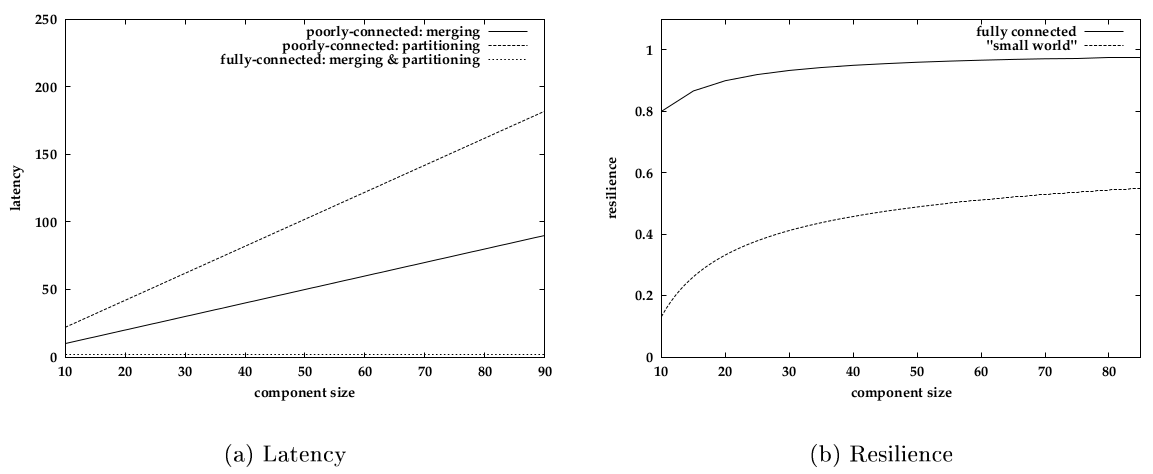
\includegraphics[scale=.4]{performance_test.png}
\caption{Simulation results}
\end{figure}

\section{Conclusion}
We have described and proved correct a hierarchical leader election algorithm using logical clocks for asynchronous dynamic networks. A set of circumstances were identified under which the algorithm does not elect a leader unnecessarily, but it remains to give a more complete characterization of such circumstances. Also, the time and message complexity of the algorithm needs to be analyzed. It would be interesting to compare the efficiency of the algorithm in the cases of perfect clocks and logical clocks.

\newpage
\bibliographystyle{unsrt}  
%\bibliography{references}  %%% Remove comment to use the external .bib file (using bibtex).
%%% and comment out the ``thebibliography'' section.


%%% Comment out this section when you \bibliography{references} is enabled.
\begin{thebibliography}{1}

\bibitem{1}
B. Awerbuch, A. Richa, and C. Scheideler.
\newblock A jamming-resistant MAC protocol for single-hop wireless networks.
\newblock In {\em In Proc. 27th ACM Symp. on Principles of Distributed Computing}, pp. 45–54, 2008.


\bibitem{2}
J. Brunekreef, J.-P. Katoen, R. Koymans, and S. Mauw.
\newblock Design and analysis of dynamic leader election protocols in broadcast networks.
\newblock {\em Distributed Computing}, 9(4):157–171, 1996.

\bibitem{3}
O. Dagdeviren and K. Erciyes.
\newblock A hierarchical leader election protocol for mobile ad hoc networks.
\newblock {\em In Proc. 8th Int’l Conf. on Computational Science, LNCS 5101}, pp. 509–518, 2008.

\bibitem{4}
A. Derhab and N. Badache.
\newblock A self-stabilizing leader election algorithm in highly dynamic ad hoc mobile networks.
\newblock {\em IEEE Trans. on Parallel and Distributed Systems}, 19(7):926–939, 2008.

\bibitem{5}
C. Fetzer and F. Cristian.
\newblock A highly available local leader election service.
\newblock {\em IEEE Trans. on Software Engineering}, , 25(5):603–618, 1999.

\bibitem{6}
E. Gafni and D. Bertsekas.
\newblock Distributed algorithms for generating loop-free routes in networks with frequently changing topology.
\newblock {\em IEEE Trans. on Communications}, C-29(1):11–18, 1981.

\bibitem{7}
Z. Haas.
\newblock  A new routing protocol for the reconfigurable wireless networks.
\newblock In {\em Proc. 6th IEEE Int’l Conf. on Universal Personal Comm.}, pp. 562–566, 1997.

\bibitem{8}
S. Han and Y. Xia.
\newblock  Optimal leader election scheme for peer-to-peer applications.
\newblock In {\em Proc. 6th Int’l. Conf. on Networking}, page 29, 2007.

\bibitem{9}
K. Hatzis, G. Pentaris, P. Spirakis, V. Tampakis, and R. Tan.
\newblock  Fundamental control algorithms in mobile networks.
\newblock In {\em Proc. 11th ACM Symp. on Parallel Algorithms and Architectures}, pp. 251–260, 1999.

\bibitem{10}
K. Hatzis, G. Pentaris, P. Spirakis, V. Tampakis, and R. Tan.
\newblock  Fundamental control algorithms in mobile networks.
\newblock In {\em Proc. 11th ACM Symp. on Parallel Algorithms and Architectures}, pp. 251–260, 1999.

\bibitem{11}
R. Ingram, P. Shields, J. Walter, and J. Welch.
\newblock An Asynchronous Leader Election Algorithm for Dynamic Networks. Technical Report 2009-1-1, Department of Computer Science and Engineering, Texas.

\bibitem{12}
L. Lamport.
\newblock  Time, Clocks, and the Ordering of Events in a Distributed System.
\newblock In {\em Communications of the ACM}, p.558, July 1978, Volume 21, Number 7.


\bibitem{13}
N. Malpani, J. Welch, and N. Vaidya.
\newblock  Leader election algorithms for mobile ad hoc networks.
\newblock In {\em Proc.ACM DIAL-M Workshop}, pp. 96–104, 2000.

\bibitem{14}
B. Mans and N. Santoro.
\newblock  Optimal Elections in Faulty Loop Networks and Applications.
\newblock {\em IEEE Trans. on Computers}, 47(3):286–297, 1998.

\bibitem{15}
S. Masum, A. Ali, and M. Bhuiyan.
\newblock  Asynchronous leader election in mobile ad hoc networks.
\newblock In {\em Proc. Int’l Conf. on Advanced Information Networking and Applications}, pp. 29–34, 2006.

\bibitem{16}
Y. Pan and G. Singh.
\newblock A fault-tolerant protocol for election in chordal-ring networks with fail-stop processor failures.
\newblock {\em IEEE Trans. on Reliability}, 46(1):11–17, 1997.

\bibitem{17}
V. Park and M. S. Corson.
\newblock A highly adaptive distributed routing algorithm for mobile wireless networks.
\newblock In {\em Proc. INFOCOM ’97}, pp. 1405–1413, 1997.

\bibitem{18}
P. Parvathipuram, V. Kumar, and G.-C. Yang.
\newblock An efficient leader election algorithm for mobile ad hoc networks.
\newblock In {\em Proc. 1st Int’l Conf. on Dist. Computing and Internet Technology, LNCS 3347}, pp. 32–41, 2004.

\bibitem{19}
M. Rahman, M. Abdullah-Al-Wadud, and O. Chae.
\newblock Performance analysis of leader election algorithms in mobile ad hoc networks.
\newblock {\em Int’l J. of Computer Science and Network Security}, 8(2):257–263, 2008.

\bibitem{20}
G. Singh.
\newblock Leader Election in the Presence of Link Failures.
\newblock {\em IEEE Trans. on Parallel and Distributed Systems}, 7(3):231–236, 1996.

\bibitem{21}
S. Stoller.
\newblock Leader election in distributed systems with crash failures.
\newblock Technical Report, Department of Computer Science, Indiana University, 1997.

\bibitem{22}
G. Tel.
\newblock {\em G. Tel. Introduction to Distributed Algorithms, Second Edition.}
\newblock Cambridge University Press, 2000.

\bibitem{23}
S. Vasudevan, J. Kurose, and D. Towsley.
\newblock Design and analysis of a leader election algorithm for mobile ad hoc networks.
\newblock In {\em In Proc.IEEE Int’l Conf. on Network Protocols}, pp. 350–360, 2004.

\bibitem{24}
Y. Wang and H. Wu.
\newblock Replication-based efficient data delivery scheme for delay/fault-tolerant mobile sensor network (dft-msn).
\newblock In {\em Proc. Pervasive Computing and Communications Workshop}, p. 5, 2006.

\bibitem{25}
R. Ingram, T. Radeva, P. Shields, S. Viqar, J.-E. Walter, and J.-L. Welch.
\newblock A Leader Election Algorithm for Dynamic Networks with Causal Clocks
\newblock , 2013.

\bibitem{26}
A. Casteigts.
\newblock JBotSim: a Tool for Fast Prototyping of Distributed Algorithms in Dynamic Networks
\newblock , 2010.


\end{thebibliography}


\end{document}
